\documentclass[
  bibliography=totoc,     % Literatur im Inhaltsverzeichnis
  captions=tableheading,  % Tabellenüberschriften
  titlepage=firstiscover, % Titelseite ist Deckblatt
]{scrartcl}

% Paket float verbessern
\usepackage{scrhack}

% Warnung, falls nochmal kompiliert werden muss
\usepackage[aux]{rerunfilecheck}

% unverzichtbare Mathe-Befehle
\usepackage{amsmath}
% viele Mathe-Symbole
\usepackage{amssymb}
% Erweiterungen für amsmath
\usepackage{mathtools}

% Fonteinstellungen
\usepackage{fontspec}
% Latin Modern Fonts werden automatisch geladen
% Alternativ zum Beispiel:
%\setromanfont{Libertinus Serif}
%\setsansfont{Libertinus Sans}
%\setmonofont{Libertinus Mono}

% Wenn man andere Schriftarten gesetzt hat,
% sollte man das Seiten-Layout neu berechnen lassen
\recalctypearea{}

% deutsche Spracheinstellungen
\usepackage{polyglossia}
\setmainlanguage{german}


\usepackage[
  math-style=ISO,    % ┐
  bold-style=ISO,    % │
  sans-style=italic, % │ ISO-Standard folgen
  nabla=upright,     % │
  partial=upright,   % ┘
  warnings-off={           % ┐
    mathtools-colon,       % │ unnötige Warnungen ausschalten
    mathtools-overbracket, % │
  },                       % ┘
]{unicode-math}

% traditionelle Fonts für Mathematik
\setmathfont{Latin Modern Math}
% Alternativ zum Beispiel:
%\setmathfont{Libertinus Math}

\setmathfont{XITS Math}[range={scr, bfscr}]
\setmathfont{XITS Math}[range={cal, bfcal}, StylisticSet=1]

% Zahlen und Einheiten
\usepackage[
  locale=DE,                   % deutsche Einstellungen
  separate-uncertainty=true,   % immer Fehler mit \pm
  per-mode=symbol-or-fraction, % / in inline math, fraction in display math
]{siunitx}

% chemische Formeln
\usepackage[
  version=4,
  math-greek=default, % ┐ mit unicode-math zusammenarbeiten
  text-greek=default, % ┘
]{mhchem}

% richtige Anführungszeichen
\usepackage[autostyle]{csquotes}

% schöne Brüche im Text
\usepackage{xfrac}

% Standardplatzierung für Floats einstellen
\usepackage{float}
\floatplacement{figure}{htbp}
\floatplacement{table}{htbp}

% Floats innerhalb einer Section halten
\usepackage[
  section, % Floats innerhalb der Section halten
  below,   % unterhalb der Section aber auf der selben Seite ist ok
]{placeins}

% Seite drehen für breite Tabellen: landscape Umgebung
\usepackage{pdflscape}

% Captions schöner machen.
\usepackage[
  labelfont=bf,        % Tabelle x: Abbildung y: ist jetzt fett
  font=small,          % Schrift etwas kleiner als Dokument
  width=0.9\textwidth, % maximale Breite einer Caption schmaler
]{caption}
% subfigure, subtable, subref
\usepackage{subcaption}

% Grafiken können eingebunden werden
\usepackage{graphicx}
% größere Variation von Dateinamen möglich
\usepackage{grffile}

% schöne Tabellen
\usepackage{booktabs}

% Verbesserungen am Schriftbild
\usepackage{microtype}

% Literaturverzeichnis
\usepackage[backend=biber, style=ieee]{biblatex}
% Quellendatenbank
\addbibresource{lit.bib}
%\addbibresource{programme.bib}

% Hyperlinks im Dokument
\usepackage[
  unicode,        % Unicode in PDF-Attributen erlauben
  pdfusetitle,    % Titel, Autoren und Datum als PDF-Attribute
  pdfcreator={},  % ┐ PDF-Attribute säubern
  pdfproducer={}, % ┘
]{hyperref}
% erweiterte Bookmarks im PDF
\usepackage{bookmark}

% Trennung von Wörtern mit Strichen
\usepackage[shortcuts]{extdash}

\author{%
  AUTOR A\\%
  \href{mailto:authorA@udo.edu}{authorA@udo.edu}%
  \texorpdfstring{\and}{,}%
  AUTOR B\\%
  \href{mailto:authorB@udo.edu}{authorB@udo.edu}%
}
\publishers{TU Dortmund – Fakultät Physik}

\begin{document}
\section{Auswertung}
\subsection{Bestimmung der Zeitkonstante über Auf- und Entladungsvorgang}
Zur Bestimmung der Zeitkonstante $RC$ werden die Messdaten wie in (\ref{tab:1})
in ein Diagramm (\ref{fig:1}) dargestellt und mit Hilfe einer linearen Ausgleichsrechnung
berechnet.
\begin{table}[H]
  \centering
  \caption{Tabelle zur Bestimmung der Zeitkonstante mit $U_\text{0}$ = $10V$}
    \begin{tabular}{c c c }
      \toprule \\
      $U_\text{c} / V$& $ln(\frac{U_\text{c}}{U_\text{0}})$ & $t /\si{\milli\second}$ \\
      \midrule \\
      10,0& -0,000 & 0,00 \\
      9,04& -0,100 & 0,10 \\
      8,48& -0,165 & 0,16 \\
      7,84& -0,243 & 0,24 \\
      7,12& -0,340 & 0,34 \\
      6,80& -0,386 & 0,40 \\
      6,16& -0,485 & 0,50 \\
      5,36& -0,624 & 0,66 \\
      4,88& -0,717 & 0,78 \\
      4,32& -0,839 & 0,96 \\
      3,76& -0,978 & 1,14 \\
      3,52& -1,044 & 1,24 \\
      3,28& -1,115 & 1,36 \\
      3,04& -1,191 & 1,50 \\
      2,72& -1,302 & 1,80 \\
      2,48& -1,394 & 2,06 \\
      2,32& -1,461 & 2,28 \\
      2,24& -1,496 & 2,50 \\
      2,16& -1,532 & 2,76 \\
      2,08& -1,570 & 3,00 \\
      2,08& -1,570 & 3,22 \\
      2,00& -1,609 & 3,38 \\
      2,00& -1,609 & 3,56 \\
      2,00& -1,609 & 3,86 \\
      2,00& -1,609 & 4,06 \\
      2,00& -1,609 & 4,30 \\
      2,00& -1,609 & 4,46 \\
      2,00& -1,609 & 4,48 \\
      2,00& -1,609 & 4,52 \\
      \bottomrule
    \end{tabular}
    \label{tab:1}
  \end{table}

\begin{figure}[H]
  \centering
  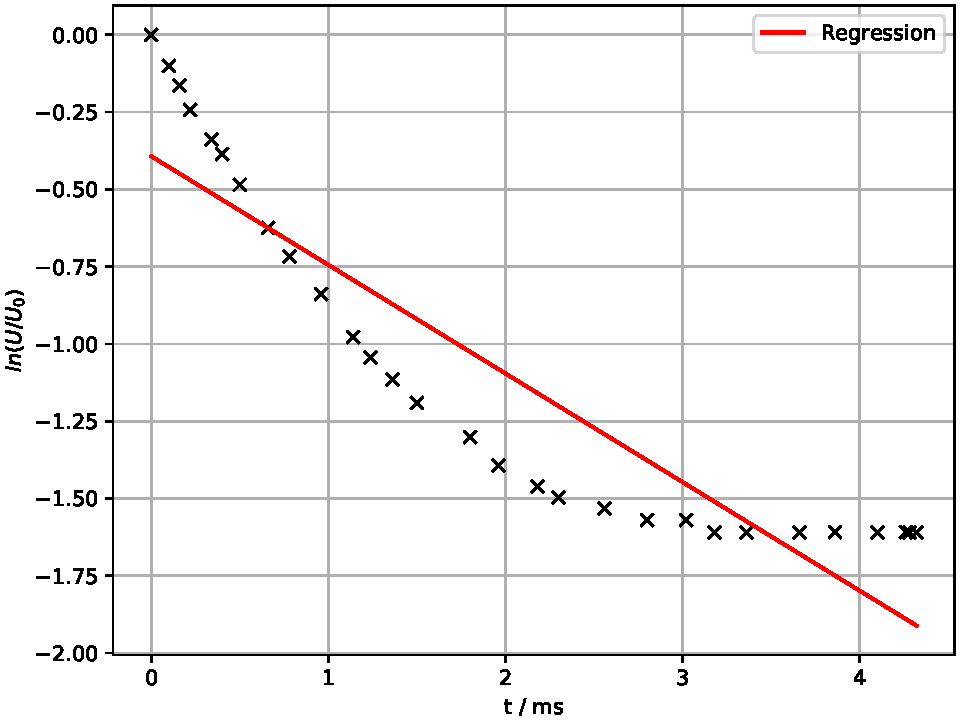
\includegraphics[width=\textwidth]{Diagramm1.pdf}
  \caption{Diagrammdarstellung}
  \label{fig:1}
\end{figure}
Die Ausgleichsrechnungs allgemein lautet:
\begin{align}
  y & = m \cdot x + b \label{eq:1}\\
  m & = \frac {\bar{xy} - \bar{x} \cdot \bar{y}} {\bar{x^2} -\bar{x}^2}&  \label{eq:2}\\
  b & = \frac {\bar{y} \cdot \bar{x}^2 - \bar{xy} \cdot \bar{x}} {\bar{x^2}-\bar{x}^2}& \label{eq:3}
\end{align}
Für diese Ausgleichsrechnung wird die Formel (\ref{eq:1}) umgeschrieben und die erechnetet Werte lautetn: \\
\newline
\centerline{$ln(\frac{U_\text{c}}{U_\text{0}}) = -\frac{1}{m} + b$}\\
\centerline{mit $m = (2,845 \pm 0,245) \cdot 10^{-3} \si{\second}$}\\
\centerline{und $b = (-0,393 \pm 0,074)$}
\newline
\end{document}
